\documentclass{standalone}
\usepackage{tikz}
\usetikzlibrary{patterns, positioning}


\begin{document}
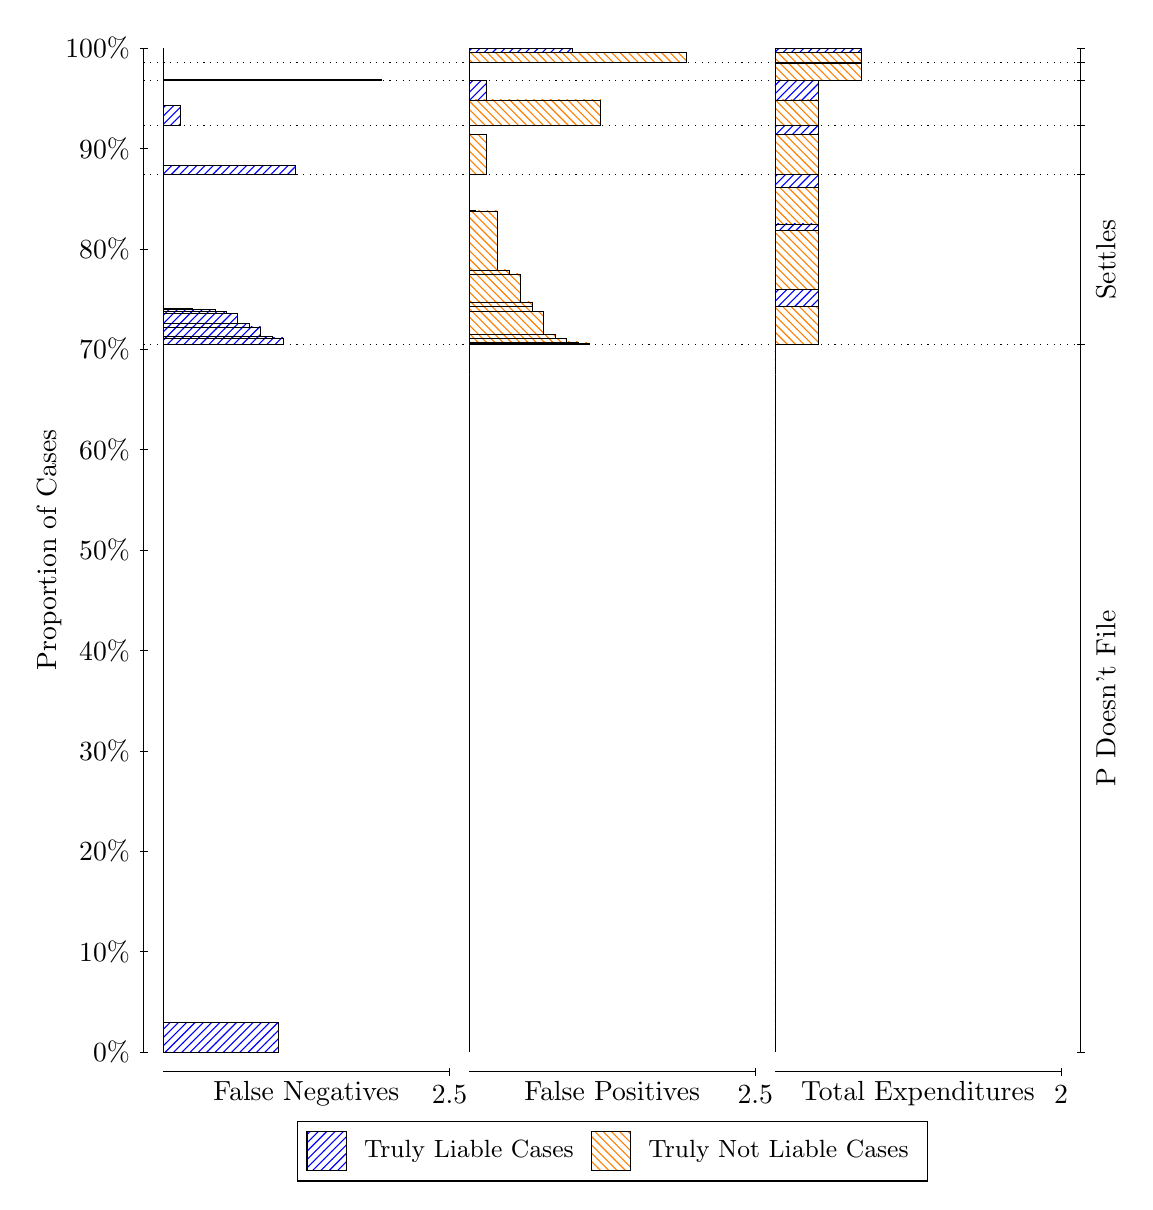
\begin{tikzpicture}
\draw[black, very thin] (1.5,1.75) -- (1.5,14.5);
\node[rotate=90, text=black, anchor=center] at (0.3, 8.125) {Proportion of Cases};
\draw[black, very thin] (1.45,1.75) -- (1.55,1.75);
\node[text=black, anchor=east] at (1.45, 1.75) {0\%};
\draw[black, very thin] (1.45,3.025) -- (1.55,3.025);
\node[text=black, anchor=east] at (1.45, 3.025) {10\%};
\draw[black, very thin] (1.45,4.3) -- (1.55,4.3);
\node[text=black, anchor=east] at (1.45, 4.3) {20\%};
\draw[black, very thin] (1.45,5.575) -- (1.55,5.575);
\node[text=black, anchor=east] at (1.45, 5.575) {30\%};
\draw[black, very thin] (1.45,6.85) -- (1.55,6.85);
\node[text=black, anchor=east] at (1.45, 6.85) {40\%};
\draw[black, very thin] (1.45,8.125) -- (1.55,8.125);
\node[text=black, anchor=east] at (1.45, 8.125) {50\%};
\draw[black, very thin] (1.45,9.4) -- (1.55,9.4);
\node[text=black, anchor=east] at (1.45, 9.4) {60\%};
\draw[black, very thin] (1.45,10.675) -- (1.55,10.675);
\node[text=black, anchor=east] at (1.45, 10.675) {70\%};
\draw[black, very thin] (1.45,11.95) -- (1.55,11.95);
\node[text=black, anchor=east] at (1.45, 11.95) {80\%};
\draw[black, very thin] (1.45,13.225) -- (1.55,13.225);
\node[text=black, anchor=east] at (1.45, 13.225) {90\%};
\draw[black, very thin] (1.45,14.5) -- (1.55,14.5);
\node[text=black, anchor=east] at (1.45, 14.5) {100\%};

\draw[black, very thin] (13.4,1.75) -- (13.4,14.5);
\draw[black, very thin] (13.35,1.75) -- (13.45,1.75);
\node[anchor=west] at (13.35, 1.75) {};
\draw[black, very thin] (13.35,10.735) -- (13.45,10.735);
\node[anchor=west] at (13.35, 10.735) {};
\draw[black, very thin] (13.35,12.892) -- (13.45,12.892);
\node[anchor=west] at (13.35, 12.892) {};
\draw[black, very thin] (13.35,13.521) -- (13.45,13.521);
\node[anchor=west] at (13.35, 13.521) {};
\draw[black, very thin] (13.35,14.087) -- (13.45,14.087);
\node[anchor=west] at (13.35, 14.087) {};
\draw[black, very thin] (13.35,14.321) -- (13.45,14.321);
\node[anchor=west] at (13.35, 14.321) {};
\draw[black, very thin] (13.35,14.5) -- (13.45,14.5);
\node[anchor=west] at (13.35, 14.5) {};

\draw[black, very thin, pattern color=blue, pattern=north east lines] (1.75,1.75) rectangle (3.2033,2.1276);
\draw[black, very thin, pattern color=orange, pattern=north west lines] (1.75,2.1276) rectangle (1.75,10.735);
\draw[black, very thin, pattern color=blue, pattern=north east lines] (1.75,10.735) rectangle (3.276,10.818);
\draw[black, very thin, pattern color=blue, pattern=north east lines] (1.75,10.818) rectangle (3.1307,10.833);
\draw[black, very thin, pattern color=blue, pattern=north east lines] (1.75,10.833) rectangle (2.9853,10.959);
\draw[black, very thin, pattern color=blue, pattern=north east lines] (1.75,10.959) rectangle (2.84,11.007);
\draw[black, very thin, pattern color=blue, pattern=north east lines] (1.75,11.007) rectangle (2.6947,11.132);
\draw[black, very thin, pattern color=blue, pattern=north east lines] (1.75,11.132) rectangle (2.5493,11.153);
\draw[black, very thin, pattern color=blue, pattern=north east lines] (1.75,11.153) rectangle (2.404,11.176);
\draw[black, very thin, pattern color=blue, pattern=north east lines] (1.75,11.176) rectangle (2.2587,11.183);
\draw[black, very thin, pattern color=blue, pattern=north east lines] (1.75,11.183) rectangle (2.1133,11.196);
\draw[black, very thin, pattern color=orange, pattern=north west lines] (1.75,11.196) rectangle (1.75,12.892);
\draw[black, very thin, pattern color=blue, pattern=north east lines] (1.75,12.892) rectangle (3.4213,13.008);
\draw[black, very thin, pattern color=orange, pattern=north west lines] (1.75,13.008) rectangle (1.75,13.521);
\draw[black, very thin, pattern color=blue, pattern=north east lines] (1.75,13.521) rectangle (1.968,13.768);
\draw[black, very thin, pattern color=orange, pattern=north west lines] (1.75,13.768) rectangle (1.75,14.087);
\draw[black, very thin, pattern color=blue, pattern=north east lines] (1.75,14.087) rectangle (4.5113,14.1);
\draw[black, very thin, pattern color=orange, pattern=north west lines] (1.75,14.1) rectangle (1.75,14.321);
\draw[black, very thin, pattern color=orange, pattern=north west lines] (1.75,14.321) rectangle (1.75,14.44);
\draw[black, very thin, pattern color=blue, pattern=north east lines] (1.75,14.44) rectangle (1.75,14.5);
\draw[black, very thin, pattern color=orange, pattern=north west lines] (5.6333,1.75) rectangle (5.6333,10.357);
\draw[black, very thin, pattern color=blue, pattern=north east lines] (5.6333,10.357) rectangle (5.6333,10.735);
\draw[black, very thin, pattern color=orange, pattern=north west lines] (5.6333,10.735) rectangle (7.1593,10.755);
\draw[black, very thin, pattern color=orange, pattern=north west lines] (5.6333,10.755) rectangle (7.014,10.768);
\draw[black, very thin, pattern color=orange, pattern=north west lines] (5.6333,10.768) rectangle (6.8687,10.816);
\draw[black, very thin, pattern color=orange, pattern=north west lines] (5.6333,10.816) rectangle (6.7233,10.864);
\draw[black, very thin, pattern color=orange, pattern=north west lines] (5.6333,10.864) rectangle (6.578,11.152);
\draw[black, very thin, pattern color=orange, pattern=north west lines] (5.6333,11.152) rectangle (6.4327,11.219);
\draw[black, very thin, pattern color=orange, pattern=north west lines] (5.6333,11.219) rectangle (6.4327,11.277);
\draw[black, very thin, pattern color=orange, pattern=north west lines] (5.6333,11.277) rectangle (6.2873,11.632);
\draw[black, very thin, pattern color=orange, pattern=north west lines] (5.6333,11.632) rectangle (6.142,11.682);
\draw[black, very thin, pattern color=orange, pattern=north west lines] (5.6333,11.682) rectangle (5.9967,12.431);
\draw[black, very thin, pattern color=blue, pattern=north east lines] (5.6333,12.431) rectangle (5.706,12.444);
\draw[black, very thin, pattern color=blue, pattern=north east lines] (5.6333,12.444) rectangle (5.6333,12.892);
\draw[black, very thin, pattern color=orange, pattern=north west lines] (5.6333,12.892) rectangle (5.8513,13.405);
\draw[black, very thin, pattern color=blue, pattern=north east lines] (5.6333,13.405) rectangle (5.6333,13.521);
\draw[black, very thin, pattern color=orange, pattern=north west lines] (5.6333,13.521) rectangle (7.3047,13.84);
\draw[black, very thin, pattern color=blue, pattern=north east lines] (5.6333,13.84) rectangle (5.8513,14.087);
\draw[black, very thin, pattern color=orange, pattern=north west lines] (5.6333,14.087) rectangle (5.6333,14.307);
\draw[black, very thin, pattern color=blue, pattern=north east lines] (5.6333,14.307) rectangle (5.6333,14.321);
\draw[black, very thin, pattern color=orange, pattern=north west lines] (5.6333,14.321) rectangle (8.3947,14.44);
\draw[black, very thin, pattern color=blue, pattern=north east lines] (5.6333,14.44) rectangle (6.9413,14.5);
\draw[black, very thin, pattern color=orange, pattern=north west lines] (9.5167,1.75) rectangle (9.5167,10.357);
\draw[black, very thin, pattern color=blue, pattern=north east lines] (9.5167,10.357) rectangle (9.5167,10.735);
\draw[black, very thin, pattern color=orange, pattern=north west lines] (9.5167,10.735) rectangle (10.062,11.219);
\draw[black, very thin, pattern color=blue, pattern=north east lines] (9.5167,11.219) rectangle (10.062,11.435);
\draw[black, very thin, pattern color=orange, pattern=north west lines] (9.5167,11.435) rectangle (10.062,12.184);
\draw[black, very thin, pattern color=blue, pattern=north east lines] (9.5167,12.184) rectangle (10.062,12.267);
\draw[black, very thin, pattern color=orange, pattern=north west lines] (9.5167,12.267) rectangle (10.062,12.73);
\draw[black, very thin, pattern color=blue, pattern=north east lines] (9.5167,12.73) rectangle (10.062,12.892);
\draw[black, very thin, pattern color=orange, pattern=north west lines] (9.5167,12.892) rectangle (10.062,13.405);
\draw[black, very thin, pattern color=blue, pattern=north east lines] (9.5167,13.405) rectangle (10.062,13.521);
\draw[black, very thin, pattern color=orange, pattern=north west lines] (9.5167,13.521) rectangle (10.062,13.84);
\draw[black, very thin, pattern color=blue, pattern=north east lines] (9.5167,13.84) rectangle (10.062,14.087);
\draw[black, very thin, pattern color=orange, pattern=north west lines] (9.5167,14.087) rectangle (10.607,14.307);
\draw[black, very thin, pattern color=blue, pattern=north east lines] (9.5167,14.307) rectangle (10.607,14.321);
\draw[black, very thin, pattern color=orange, pattern=north west lines] (9.5167,14.321) rectangle (10.607,14.44);
\draw[black, very thin, pattern color=blue, pattern=north east lines] (9.5167,14.44) rectangle (10.607,14.5);
\draw[black, dotted] (1.5,10.735) -- (13.4,10.735);
\draw[black, dotted] (1.5,12.892) -- (13.4,12.892);
\draw[black, dotted] (1.5,13.521) -- (13.4,13.521);
\draw[black, dotted] (1.5,14.087) -- (13.4,14.087);
\draw[black, dotted] (1.5,14.321) -- (13.4,14.321);
\draw[black, very thin] (1.75,1.5) -- (5.3833,1.5);
\node[text=black, anchor=north] at (3.5667, 1.5) {False Negatives};
\draw[black, very thin] (5.3833,1.45) -- (5.3833,1.55);
\node[text=black, anchor=north] at (5.3833, 1.45) {2.5};

\draw[black, very thin] (5.6333,1.5) -- (9.2667,1.5);
\node[text=black, anchor=north] at (7.45, 1.5) {False Positives};
\draw[black, very thin] (9.2667,1.45) -- (9.2667,1.55);
\node[text=black, anchor=north] at (9.2667, 1.45) {2.5};

\draw[black, very thin] (9.5167,1.5) -- (13.15,1.5);
\node[text=black, anchor=north] at (11.333, 1.5) {Total Expenditures};
\draw[black, very thin] (13.15,1.45) -- (13.15,1.55);
\node[text=black, anchor=north] at (13.15, 1.45) {2};

\node[text=black, centered, rotate=90] at (13.72, 6.2424) {P Doesn't File};
\node[text=black, centered, rotate=90] at (13.72, 11.814) {Settles};





\draw (7.449999999999999,1.5) node[draw=none] (baseCoordinate) {};
\begin{scope}[align=center]
        \matrix[scale=0.5, draw=black, below=0.5cm of baseCoordinate, nodes={draw}, column sep=0.1cm]{
            \node[rectangle, draw, minimum width=0.5cm, minimum height=0.5cm, pattern color=blue, pattern=north east lines] {}; &
            \node[draw=none, font=\small, text=black] (B) {Truly Liable Cases}; &
            \node[rectangle, draw, minimum width=0.5cm, minimum height=0.5cm, pattern color=orange, pattern=north west lines] {}; &
            \node[draw=none, font=\small, text=black] (B) {Truly Not Liable Cases}; \\
            };
\end{scope}

\end{tikzpicture}
\end{document}